\documentclass[a4paper, titlepage, 12pt]{article}
\usepackage[a4paper, margin=2.2cm]{geometry}
\usepackage[utf8]{inputenc}
\usepackage{float, amssymb, amsmath, amsbsy} 
\usepackage{mathdots, mathrsfs, topcapt, multirow}
\usepackage[hidelinks]{hyperref}
\usepackage{graphicx, caption, booktabs}
\usepackage{subfigure}
\usepackage[spanish, es-tabla]{babel}
\usepackage{mathtools, fancyref}
\usepackage{multicol}
\usepackage[x11names,table]{xcolor}
\usepackage{listings}
\usepackage{tikz}
\usepackage{multicol}
\usepackage{amsthm}
\def\proof{\paragraph{Demostraci\'on:\\}}
\def\endproof{\hfill$\blacksquare$}

\newtheorem{thm}{Teorema}[section]


\theoremstyle{definition}%Pone en letra negrita la palabra proposicion,etc 

\newtheorem{de}[thm]{Definición}
\newtheorem{nota}[thm]{Nota}
\newtheorem{ej}[thm]{Ejemplos}
\newtheorem{reco}[thm]{Recordatorio}
\newtheorem{com}[thm]{Comentario}



\theoremstyle{Teorema}   

\newtheorem{prop}[thm]{Proposición}
\newtheorem{teo}[thm]{Teorema}
\newtheorem{coro}[thm]{Corolario}
\newtheorem{lema}[thm]{Lema}
\newtheorem{obs}[thm]{Observación}



\theoremstyle{break}

\newtheorem{demo}{Demostración} % (no lo uso...solo era para probar)


\title{\textbf{Fibonacci Heap aplicado al algoritmo de Dijkstra y Prim}\\
  \vspace{2.5cm}
  \textsc{Facultad de Ciencias, UNAM}\\
  \normalsize\textsc{Programación Declarativa, 2021-1}
}

\author{ Villegas Salvador Kevin Ricardo }

\begin{document}
\maketitle

\section{Preliminares}
\subsection{Especificaciones}
Se presentan las herramientas utilizadas para la construcción del sistema,
modulos utilizados para llevar acabo la resolución del problema, así como las pruebas del 
algoritmo.
\subsubsection{Herramientas}
\begin{itemize}
  \item \textbf{Lenguaje de Programación.}\\
  Haskell
  \item \textbf{Sistema de Construcción.}\\
  Cabal (The Common Architecture for Building Applications and Libraries) 2.4.0.0
  \item \textbf{Documentación.}\\
  Haddock 2.22.0
  \item \textbf{Control de versiones.}\\
  GitHub 2.30.0 \href{https://github.com/ciencias-unam/proyecto-final-kevRicardo}{Fibonacci Heap (Dijkstra y Prim)}
\end{itemize}
\subsubsection*{Estructura}
En conjunto con \textbf{Cabal} se realizó la construcción del directorio de la siguiente manera:
\begin{center}
  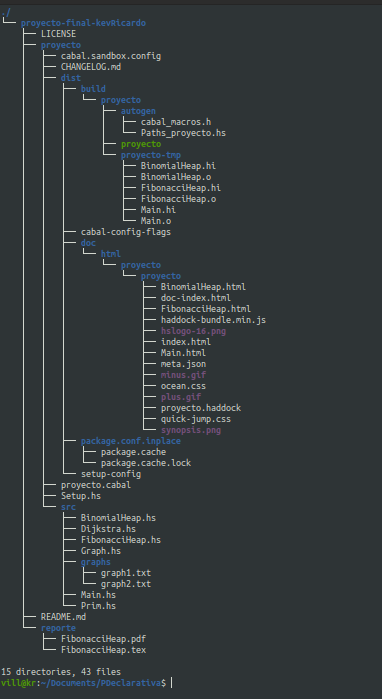
\includegraphics[scale=.5]{img/treepath.png}
\end{center}

Dentro de la carpeta \textbf{./reporte} podemos encontrar, éste archivo. Seguido de la carpeta \textbf{./proyecto} donde 
se encuentra todo lo relacionado con el sistema.\\

Ahora bien seguimos con la siguiente estructura:
\begin{itemize}
  \item \textbf{./dist/build}. Se encuentra el archivo ejecutable.
  \item \textbf{./dist/doc}. La documentación del sistema.
  \item \textbf{./src}. Código fuente
  \item Seguido de la configuraciónes necesarias para poder correr el código
\end{itemize}

\subsection{Manejo del sistema}
\subsubsection*{Descarga del proyecto}
El proyecto se puede encontrar en la siguiente liga: \textit{\href{https://github.com/ciencias-unam/proyecto-final-kevRicardo}{https://github.com/ciencias-unam/proyecto-final-kevRicardo}}. 
Para descargarlo basta con ejecutar \textit{Git} en cualquier directorio del sistema de archivos.\\
\small
\begin{lstlisting}
  $ https://github.com/ciencias-unam/proyecto-final-kevRicardo.git
\end{lstlisting}
\subsubsection*{Compilación y ejecución}
Para poder compilar el proyecto se dará por hecho que ya se tiene \textsc{Cabal} instalado, de lo contrario podrá ejecutar 
\begin{lstlisting}
  $ sudo apt-get install cabal-install
\end{lstlisting}
Una vez ejecutado el comando, podrá ejecutar lo siguiente para poder si \textsc{Cabal} se ha instalado correctamente
\begin{lstlisting}
  $ cabal --version
\end{lstlisting}

Una vez ya teniendo todo listo, podemos comenzar la compilación, y ejecución del programa. Primero nos posicionamos en la ruta
\begin{lstlisting}
  .../PDeclarativa/proyecto-final-kevRicardo/proyecto$
\end{lstlisting}
Ya que estamos en la ruta correcta, para obtener el archivo ejecutable, ponemos el siguiente comando:
\begin{lstlisting}
  .../proyecto-final-kevRicardo/proyecto$ cabal build
\end{lstlisting}
Esto nos generará el ejecutable en la dirección \textit{./dist/buil/proyecto}.
Una vez generado nuestro ejecutable, podemos correr el proyecto con el siguiente comando:
\begin{lstlisting}
  .../proyecto-final-kevRicardo/proyecto$ cabal run
\end{lstlisting}
Cabe mencionar que no es necesario, realizar el ejecutable antes de correr el proyecto, ya que run, lo genera por sí solo.
Para generar la documentación del proyecto, utilizamos el siguiente comando:
\begin{lstlisting}
  .../proyecto-final-kevRicardo/proyecto$ cabal haddock --executables
\end{lstlisting}
Así la documentación la encontramos en \textit{./dist/doc/html/proyecto/proyecto/}\\

Una vez ya corriendo el proyecto empezará por pedir los archivos a procesar para poder probar el algoritmo de Dijkstra y Prim 
usando Fibonacci Heap.
\end{document}